

This literature review serves to provide the essential technical and theoretical background underpinning the methodology employed in this thesis. It delves into the core concepts and established techniques within the fields of remote sensing and machine learning that are pertinent to this research for the identification and classification of small water reservoirs from satellite imagery. By reviewing the relevant literature in this field, I will pinpoint the precise knowledge gap, namely the absence of a validated, end-to-end pipeline tailored for high-resolution detection of small farm reservoirs in East England.

The following sections build on this foundation:
\begin{enumerate}
    \item \textbf{Remote Sensing for Water Body Mapping} - Why optical satellites (Sentinel-2, Landsat) are ideal for small-reservoir mapping, comparing their spatial, spectral and revisit capabilities.
    \item \textbf{Water Detection Methods} - Techniques for isolating water pixels including classic, numerically computed indices (NDWI, MNDWI, AWEI-NSH/SH), traditional classifiers (SVM, Maximum Likelihood), and deep-learning algorithms.
    \item \textbf{Cloud Detection and Masking} - From simple quality-flag masks to Fmask’s object-based approach and OmniCloudMask’s sensor-agnostic neural model, and how each handles cloud/shadow errors.
    \item \textbf{Machine Learning Algorithms} - Overview of unsupervised clustering versus supervised learning, with a comparison focused on the practical applications of Random Forest and Keras Sequential.
    \item \textbf{Machine Learning and Water Classification}
    \begin{enumerate}
        \item How supervised methods have been applied to remote-sensing water detection.  
        \item Key case studies of reservoir mapping, and where existing pipelines still fall short.
    \end{enumerate}
\end{enumerate}

By reviewing these interconnected topics, this literature review aims to build a comprehensive understanding of the technical landscape, providing the necessary foundation for the methodology developed and applied in this thesis.

\section{Remote Sensing for Water Body Mapping}
\subsection{What is Remote Sensing?}
Remote sensing is the practice of acquiring information about the Earth's surface without direct contact, typically through sensors mounted on satellites or aircraft \citep{usgs_2022a}. By capturing the reflected or emitted electromagnetic radiation from land, water, and atmosphere, remote sensing provides systematic, repeatable, and scalable observations across large areas.

For the task of small reservoir detection, optical satellite imagery is particularly well-suited. Optical sensors measure reflected solar radiation in visible, near-infrared, and shortwave-infrared wavelengths, enabling strong discrimination between surface water and surrounding land cover based on spectral signatures. Water bodies typically appear darker in the near-infrared and shortwave-infrared bands compared to vegetation, soil, or built-up areas, making them distinguishable through simple band ratios or more advanced machine learning methods.

\subsection{Satellite Options}
There are several options for optical satellites currently in operation. The first requirement for this study is that the data must be freely available, otherwise it would be unfeasible to scale the project globally without significant monetary investment. This means that the ultra-high resolution satellite imaging platforms such as MAXAR are not option as they are privately run and therefore have costs for their use. The two main remaining options are to use Sentinel, the European Space Agency (ESA) satellites, or Landsat, the NASA satellites, both of which are publicly funded and host freely accessible data.

The Sentinel 2 constellation is made up of three satellite: Sentinel 2A, 2B, and 2C, with the Sentinel 2A, the first to be launched, operating since 2015 \citep{esa_2024}. Each satellite has functionally the same sensors and specifications, so whenever "Sentinel 2" is mentioned in this thesis, this is used as an umbrella term to mean any of the three Sentinel 2 satellites. These satellites have a maximum spatial resolution of 10m, with file options for 20m and 60m files. 

Landsat 7 has been operating since 1999, however due to the failure of a component called the Scan Line Corrector in 2003, images have had "gaps" in them \citep{usgs_2024}. Landsat 8 and 9 operate as intended and have been in orbit since 2013 and 2021 respectively \citep{usgs_2023, usgs_2022}. These satellites have a maximum spatial resolution of 30m, which is considerably less fine than the Sentinel 2 options. For this reason, many researchers prefer to use Sentinel images over Landsat as the additional detail afforded by Sentinel is necessary for many applications \citep{ghansah_2022_monitoring, kirby_ferguson_rennie_cousineau_nistor_2024}. 

\subsection{Resolution}
There are two different kinds of resolution to consider when discussing remote sensing data. The first is the regular, pixel resolution, just like the one on televisions, and computer or phone screens. This resolution is calculated from the product of the number of pixels on each length of the image, so an image with 1920 pixels along its length and 1080 pixels along its width has a 1920x1080 resolution, and a total pixel count of 2,073,600. This is also known as "full HD" \citep{lenovo_2021}. 

The second kind of resolution is specific to satellite imagery and it is known as "spatial resolution". This is defined as the "scale or size of the smallest unit of an image capable of distinguishing objects" \citep{zhang_li_zhang_li_2023}. When we say "10 metre resolution", this means the spatial resolution of satellite image, meaning each pixel on the image represents a 10m by 10m area on the ground. 

Technically speaking, resolution is defined by the peaks of the reflecting light from an object not overlapping with the nearest light-reflecting object that can be resolved as well. This is shown in figure \ref{fig:LR resolution graph} and this principle applies to various fields of optical imaging. 

\begin{figure}[ht]
    \centering
    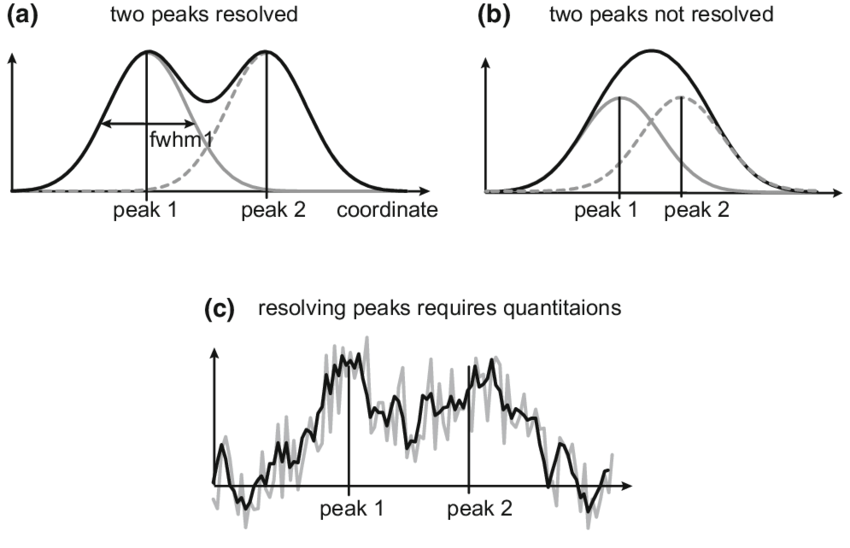
\includegraphics[width=0.6\textwidth]{contents/figures/LR resolution peaks.jpg}
    \caption{Graphical representation of resolution \citep{kudryashev_2018}}
    \label{fig:LR resolution graph}
\end{figure}

It is important to note that satellite images have a spatial resolution but they also have a regular pixel resolution. For example, the highest resolution Sentinel 2 satellite images used in the development of software for this study (the ones with 10m spatial resolution) have a pixel resolution of 10980x10980, meaning a total pixel count of 120,560,400. This very large pixel count is necessary to be able to zoom in very close to see small features on the ground for Sentinel 2 satellites, which orbit at 786 km \citep{esa_2023}. 

\subsection{Optical Sensors}
There are thirteen optical imaging sensors on the Sentinel 2 satellites \citep{sinergise_2025}. These sensors have varying spatial resolutions, ranging from 10m for the sharpest and largest images, and 60m for the smallest images with the least detail. The 60m resolution images are not detailed enough to be usable for data labelling or model training, however they are useful for fast troubleshooting as the smaller files take less time to open and manipulate. Images generated with 10m or 20m resolution are usable, however 10m resolution is preferred for easier viewing. 

\section{Water Detection Methods}
\subsection{Spectral Water Indices}
Spectral water indices play a pivotal role in distinguishing water pixels from surrounding land cover. These band-ratio techniques have become standard in operational water mapping workflows, offering enhanced contrast between water and non-water surfaces across diverse environments. 

\subsubsection{Normalised Difference Water Index}
The Normalised Difference Water Index (NDWI), introduced by \cite{mcfeeters_k_1996}, uses the green and near-infrared bands (NIR) to delineate water features from other land areas. 

\begin{equation} \label{eq-ndwi}
NDWI = \frac{\rho_{green} - \rho_{NIR}}{\rho_{green} + \rho_{NIR}}
\end{equation}

For a computer, equation \ref{eq-ndwi} means that, to calculate one pixel for a map of NDWI from a satellite image, it must take the corresponding pixel in the image for green reflectance, and the corresponding pixel in the image for NIR reflectance, and apply the equation to it. In reality, although this is the process what would be most intuitive to humans, computers perform significantly better when they take advantage of matrix-wise operations to vastly improve efficiency, so rather than calculating a NDWI array by going pixel by pixel and applying the equation to each one, computers conduct all the calculations at the same time. This same method applies for each other index that will be discussed. More details on this method will be discussed further in the methodology section. 

\subsubsection{Modified Normalised Difference Water Index}
The Modified NDWI (MNDWI) replaces the NIR band in NDWI with a short-wave infrared band (SWIR) to suppress built-up and vegetated noise \citep{xu_hanqiu_2006}. 

\begin{equation} \label{eq-mndwi}
MNDWI = \frac{\rho_{green} - \rho_{SWIR1}}{\rho_{green} + \rho_{SWIR1}}
\end{equation}

Sentinel 2 has two SWIR bands, and MNDWI specifically requires the SWIR1 band, which has a 20m spatial resolution. 

\subsubsection{Automated Water Extraction Index}
There are also some newer spectral water indices that have been used for water detection, including the Automated Water Extraction Index (AWEI) \citep{feyisa_gudina_meilby_fensholt_proud_2014b}, which has two forms: one optimised for higher-accuracy detection of water in shadowed regions, and another for unshadowed regions, AWEI-SH and AWEI-NSH respectively.

\begin{equation}
AWEI_{NSH} = 4 \times (\rho_{green} - \rho_{SWIR1}) - (0.25 \times \rho_{NIR} + 2.75 \times \rho_{SWIR2})
\end{equation}

\begin{equation}
AWEI_{SH} = \rho_{green} + 2.5 \times \rho_{blue} - 1.5 \times (\rho_{NIR} + \rho_{SWIR1}) - 0.25 \times \rho_{SWIR2}
\end{equation}

These indices are slightly more complex than NDWI and MNDWI and make use of different bands, such as the blue band, which has a 10m spatial resolution, and the SWIR2 band, which has a 20m spatial resolution. 

Both the study conceiving this index \citep{feyisa_gudina_meilby_fensholt_proud_2014b} and independent studies comparing various index performances \citep{kirby_ferguson_rennie_cousineau_nistor_2024} have shown that AWEI, specifically AWEI-NSH generally outperforms the other methods of spectral index water delineation. 

\subsection{Traditional Machine Learning Methods}
Another method of identifying water pixels in an image is to use machine learning (ML). The algorithms discussed in this sub-section are both supervised algorithms, meaning they ingest labelled training data and output a prediction on the class of each pixel in an image. These types of algorithms are significantly more complex than a simple spectral water index as they require training and often precise fine-tuning for optimal results \citep{vapnik_vladimir_n_1997}. However, ML algorithms are also often more accurate when trained on enough data. ML algorithms can model complex, multi-feature relationships for higher accuracy, while indices use simpler, although often significantly faster formulas based on fewer spectral bands.

\subsubsection{Support Vector Machine}
Support Vector Machine (SVM) is a supervised ML algorithm with the goal being to find an optimal hyperplane that best separates data points belonging to different classes in a high-dimensional space \citep{berwick_2003}. A hyperplane is essentially a decision boundary; in 2D, it is a line, in 3D it is a plane, and in higher dimensions, it is a hyperplane \citep{ktena_sotiras_ferrante_schirmer_arichi_chung_2023}. It maximises the margin between the hyperplane and the nearest points (support vectors) for robust classification.

SVM has been tested on accuracy of water detection, \citep{maity_2016} as well as vegetation and urban areas. 

\begin{table}[ht]
    \centering
    \begin{tabular}{|l|c|c|c|}
        \hline
        CLASS & Urban & Vegetation & Water \\
        \hline
        Urban & 72.53 & 0.25 & 27.22 \\
        Vegetation & 0 & 97.70 & 2.30 \\
        Water & 10.53 & 6.17 & 83.30 \\
        \hline
    \end{tabular}
    \caption{SVM Confusion Matrix \citep{maity_2016}}
    \label{tab:LR SVM confusion matrix}
\end{table}

In table \ref{tab:LR SVM confusion matrix}, the numbers along the diagonal (i.e. the where "urban" meets "urban", the cell where "vegetation" meets "vegetation", and the cell "water" meets "water") show the correct predictions made by the SVM model, or true positives, whereas the ones off the diagonal show misclassification, or false positives. While SVM has a high accuracy, as is shown by the values along the diagonal, the best application for it seems to be in identifying vegetation, where it achieves up to 97.7\% accuracy with relatively few false positives and false negatives. However, when identifying water, the accuracy falls to 83.3\%, with false negatives and false positives reaching up to 27.2\%. 

\begin{itemize}
    \item \textbf{Advantages:}
    \begin{itemize}
        \item Effectively handles high-dimensional data and complex non-linear separations using kernels.
        \item Often achieves greater accuracy, particularly where features have similar spectral responses.
    \end{itemize}
    \item \textbf{Disadvantages:}
    \begin{itemize}
        \item Requires labelled training data and significant computational resources, especially for training.
        \item Can be less interpretable and needs careful parameter tuning compared to simple index thresholds.
        \item More complex implementation, especially over spectral indices.
    \end{itemize}
\end{itemize}

\subsubsection{Maximum Likelihood Classifier}
Similarly to SVM, the Maximum Likelihood Classifier (MLC) is a supervised ML algorithm. MLC uses probability distributions to assign data points a class. It assumes data within each class follows a normal distribution and uses training data to estimate the probability parameters for each class \citep{arcmap_2021}. 

In remote sensing specifically, MLC classifies pixels in satellite imagery by calculating the probability that the pixel's spectral signature belongs to each predefined land cover class, assigning it to the most probable one.

\begin{itemize}
    \item \textbf{Advantages:}
    \begin{itemize}
        \item Considers class variability (variance-covariance) across all input bands, often yielding robust results.
        \item Provides quantitative probability values for pixel assignment to each class.
    \end{itemize}
    \item \textbf{Disadvantages:}
    \begin{itemize}
        \item Requires training data and more computational resources.
        \item Assumes normal distribution for class data, which can limit accuracy if untrue.
        \item Sensitive to the quality and representativeness of training data; poorly defined training sites significantly impact results.
        \item Also more complex to implement than spectral indices.
    \end{itemize}
\end{itemize}

\subsection{Deep Learning Methods}
\subsubsection{OmniWaterMask}
OmniWaterMask is a Python library designed for high-accuracy water segmentation in satellite imagery \citep{dpird-dma_2024}. It supports imagery from various satellites, crucially Sentinel 2, but also higher resolution options such as MAXAR, and is built on data from the Red, Green, Blue, and NIR bands. Importantly, these are the four bands on Sentinel 2 that have access to the 10m resolution sensors. 

The documentation for OmniWaterMask claims it provides "high accuracy" water segmentation. However, unlike other products for deep learning solutions to remote sensing problems from the Department of Primary Industries and Regional Development \citep{wright_2025}, OmniWaterMask does not yet have scientific paper published to evaluate its accuracy. As a result, this approach has not been compared to any other approaches such as spectral index water detection or traditional machine learning, meaning that a direct quantitative comparison of OmniWaterMask's accuracy is not available.

\subsection{Resolution Considerations}
It is important to note that the selection of the "best" index for this project does not solely depend on the accuracy with which the index can delineate boundaries of water or total area. A large part of this project is made up of data labelling and training point digitisation, meaning that the viewing experience should be taken into account. 

Only four of the thirteen optical imaging sensors on Sentinel 2 can achieve the maximum 10m spatial resolution: Band 2 (blue), Band 3 (green), Band 4 (red), and Band 8 (near-infrared). 

\begin{table}[ht]
\centering
\begin{tabular}{|c|c|c|c|}
\hline
\textbf{Band} & \textbf{Label} & \textbf{Wavelength (nm)} & \textbf{Resolution (m)} \\
\hline
1 & Aerosol & 443 & 60 \\
\rowcolor{yellow} 2 & Blue & 490 & 10 \\
\rowcolor{yellow} 3 & Green & 560 & 10 \\
\rowcolor{yellow} 4 & Red & 665 & 10 \\
5 & Red Edge & 705 & 20 \\
6 & Red Edge & 740 & 20 \\
7 & Red Edge & 783 & 20 \\
\rowcolor{yellow} 8 & NIR & 842 & 10 \\
8A & Narrow NIR & 865 & 20 \\
9 & Water Vapour & 945 & 60 \\
10 & SWIR Cirrus & 1375 & 60 \\
11 & SWIR 1 & 1610 & 20 \\
12 & SWIR 2 & 2190 & 20 \\
\hline
\end{tabular}
\caption{Sentinel 2 Spectral Bands Information \citep{sinergise_2025}}
\end{table}

As will be covered in more depth in the methodology section, the way that spectral indices must be calculated involves ensuring all arrays converted from an image must be of the same size. This means that, if an index is calculated using two bands of different resolutions, the lower resolution band takes precedent, resulting in a lower resolution image. Given that MNDWI, AWEI-SH, and AWEI-NSH all require at least one band with 20m resolution, every image generated displaying any of these water will have roughly half the resolution of an image generated using NDWI. This is because NDWI uses only the green and NIR bands, both of which are supported with 10m resolution. 

\begin{figure}[ht]
     \centering
     \begin{subfigure}[b]{0.45\textwidth}
         \centering
         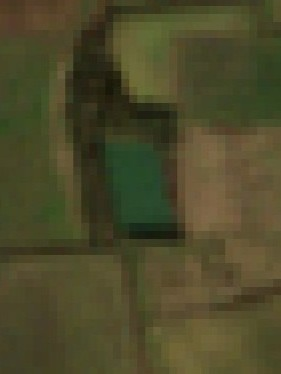
\includegraphics[width=\textwidth]{contents/figures/LR 10m res.jpg}
         \caption{10m Resolution Example}
         \label{fig:10m resolution example}
     \end{subfigure}
     \hfill
     \begin{subfigure}[b]{0.45\textwidth}
         \centering
         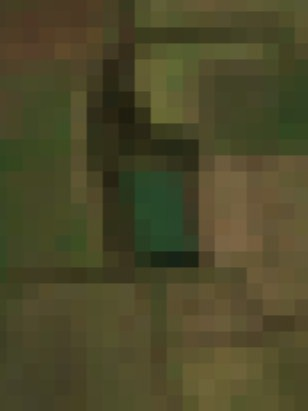
\includegraphics[width=\textwidth]{contents/figures/LR 20m res.jpg}
         \caption{20m Resolution Example}
         \label{fig:20m resolution example}
     \end{subfigure}
        \caption{10m (left) vs 20m (right) Resolution Comparison for a True Colour Image (TCI)}
        \label{fig:lit review resolution comparison}
\end{figure}

A higher resolution image is sharper and clearer than one with lower resolution, as can be seen from figure \ref{fig:lit review resolution comparison} comparing the appearance of a reservoir in a 10m spatial resolution image against a 20m spatial resolution image. This makes it easier to spot small details on a screen, as well as having the advantage of reducing eye strain when looking at screens for a long time \citep{klein_2024}. Given that the data labelling and training point digitisation process involves careful observation of these images on computer screens for extended periods of time, an index capable of accessing higher resolutions is a non-trivial consideration. Additionally, as this project is concerned with the detection of small reservoirs, it is most natural to give priority to the images that have the most information in them. 

Therefore, although not explicitly related to the performance of the index, NDWI does have the resolution advantage over the other indices.

\subsection{Summary}
Studies by \cite{kirby_ferguson_rennie_cousineau_nistor_2024} comparing water detection performance across spectral indices and machine learning methods found that, while no single index is universally best for identifying water in satellite imagery, AWEI-NSH performed most successfully in the tested study locations. MNDWI did not perform as well as NDWI in many cases, and the AWEI-SH index performed worse than AWEI-NSH in general as well. 

Out of the machine learning methods, SVM was the most performant overall, however MLC was better suited for delineating areas of water, rather than boundaries. This is important for the application in this project because it is concerned with spotting water reservoirs, which would benefit from identifying an area, rather than identifying the delineation from water to land, for example. 

To help visualise the basic sensitivity analysis conducted for selecting which method to select, table \ref{tab:water detection comparisons} shows each method of water detection discussed along with the expected complexity of implementation and the expected effectiveness of the method at detecting water once implemented, based on the quantitative comparative study by \cite{kirby_ferguson_rennie_cousineau_nistor_2024}.

\begin{table}[ht]
\centering
\begin{tabular}{|c|c|c|c|}
\hline
\textbf{Method} & \textbf{Type} & \textbf{Complexity} & \textbf{Effectiveness} \\
\hline
Spectral Index & NDWI & Simple & Moderate \\
Spectral Index & MNDWI & Simple & Low \\
Spectral Index & AWEI-SH & Simple & Moderate \\
Spectral Index & AWEI-NSH & Simple & High \\
Traditional ML & SVM & High & High \\
Traditional ML & MLC & High & Moderate \\
Deep Learning & OmniWaterMask & High & Unverified \\
\hline
\end{tabular}
\caption{Comparison of different water detection methods in expected complexity of implementation and expected effectiveness}
\label{tab:water detection comparisons}
\end{table}

Given that each of the spectral indices are simple equations and Python's integration with NumPy makes large matrix-wise operations very efficient and straightforward, it is logical that their implementation would be straightforward as well. This will be discussed further in the methodology section. 

Although MLC uses more advanced probability measures to produce a likelihood that a given pixel is or is not water, spectral indices produce high or low values depending on how much of the required wavelengths are reflected. This could behave as a kind of "confidence" or likelihood that a given pixel is water. 

The deep learning and traditional machine learning methods, however, are much more complex, and would require significant time investment to fully understand and apply properly. 

\section{Cloud Detection and Masking}
Clouds and their shadows can be misclassified as water bodies or reservoirs, so cloud contamination presents one of the potential obstacles in optical water mapping. There are several possible approaches of varying complexity and effectiveness when considering optimal methods of cloud masking. 

\subsection{QI Correspondence Method}
The most basic method makes use of the "Quality Indicator" (QI) files stored in each Sentinel 2 image \citep{gatti_bertolini_carriero_2015}. These files are "XML reports including Quality Indicators, GML Quality Mask files and JP2 Preview Image file". One of the quality mask files named "MSK\_CLDPRB\_20m" contains data for each pixel on the likelihood of that pixel being a cloud pixel. This likelihood is expressed as a float number between 0 and 1, 0 being not a cloud, and 1 being almost assuredly a cloud. 

By using these files to eliminate the corresponding pixels in the band images, we can  conduct basic cloud masking. This approach is basic, but very easy to implement, making it likely well-suited for a study where cloud cover is low. 

As there was no previous literature on this masking method, I have named it the "QI Correspondence" method as it stores cloud pixel positions using the QI cloud masking file, and then eliminates the corresponding pixel in the band images by converting it to a \texttt{Not a Number} (\texttt{NaN}).

\subsection{FMask}
Although initially designed exclusively for Landsat, \cite{frantz_haß_uhl_stoffels_hill_2018} was able to replace the missing thermal imaging sensor required for Landsat, enabling FMask to be adapted for Sentinel. The Fmask algorithm and its subsequent versions have set the benchmark for automated, object-based cloud and cloud-shadow detection in Landsat imagery \citep{qiu_zhu_he_2019}. 

The Fmask (Function of mask) algorithm is a single-date, object-based method for detecting clouds and their shadows in optical satellite images \citep{tarrio_tang_masek_claverie_ju_qiu_zhu_woodcock_2020}. It first uses a series of spectral tests, examining the reflectance characteristics that distinguish clouds from land and water, and computes a cloud probability layer based on measures of brightness and how much the spectrum varies. Pixels flagged as potential clouds are then grouped into spatial objects, and the algorithm uses thermal measurements to estimate each cloud’s height \citep{zhu_helmer_2018}. By projecting the three-dimensional shape of each cloud along the sun’s path, Fmask defines where its shadow should fall, and then confirms actual shadow pixels by looking for darker targets in those areas. In the same pass it also identifies snow and water bodies using additional spectral criteria. The result is a per-pixel map assigning each location to one of five classes: clear sky, cloud, cloud shadow, snow, or water. Downstream workflows then use these classes to restrict analysis to clear-sky pixels and thus greatly reduce errors when extracting water bodies. 

\subsection{OmniCloudMask}
OmniCloudMask is built around a deep convolutional neural network that learns to label each pixel as either clear sky, clouded, or under the shadow of a cloud \citep{wright_duncan_nik_thompson_george_2024}. During training, the input patches of red, green and near-infrared bands are first spectrally normalised and then randomly resampled to resolutions between ten and fifty meters. This “mixed-resolution” approach allows the network to be trained on the spectral and spatial characteristics of both medium and high resolution sensors. 

The model’s final layers perform a three-way classification on each pixel, and new images are normalised and resized then fed into the network in overlapping tiles. This allows the model to be trained on features that do not depend on the sensor's characteristics, meaning that it can make predictions on data from a very wide range of satellite imaging platforms without needing to be trained individually to that platform. 

\subsection{Summary}
The FMask and OmniCloudMask algorithms are built on sophisticated and long-standing platforms which are being constantly maintained. This allows them to offer higher accuracy than the basic QI Correspondence method, however this comes at the cost of more complex implementation and computationally expensive operations. 

\begin{table}[ht]
\centering
\begin{tabular}{|c|c|c|c|}
\hline
\textbf{Method} & \textbf{Type} & \textbf{Complexity} & \textbf{Effectiveness} \\
\hline
QI Correspondence & Numerical & Simple & Unverified \\
FMask & MNDWI & Moderate & High \\
Deep Learning & OmniCloudMask & Moderate & Moderate \\
\hline
\end{tabular}
\caption{Comparison of different cloud masking methods in complexity of implementation and expected effectiveness}
\label{tab:cloud masking comparisons}
\end{table}

The QI Correspondence method is very simple and easy to implement but likely does not offer particularly high accuracy. However, for the specified month of March 2025, having very low cloud cover, a high-accuracy model may not be required, and for a project of this scope, it could be more beneficial to accept the accuracy loss with the QI Correspondence method, and to dedicate that time for the problems that need solving in the machine learning or software program development sections. 

\section{Machine Learning Algorithms}
Much work and research has been carried out in the machine learning sector, so the benefits, as well as the disadvantages, are well understood. Computer algorithms as a whole are used to sift through large quantities of data which would otherwise be too large for a human to individually examine. Some sophisticated machine learning algorithms offer the specific advantage of “on the job improvement” \citep{zhang_2010_new}. This means that, as the classification model scans more images, it learns more and more about the content of those pictures, and the lessons learned from this can be fed back into itself, thereby improving its overall accuracy constantly. However, most other computer algorithms may rely on constant human intervention or extensive training data. 

There are different kinds of machine learning algorithms. The two main subsets are "supervised" and "unsupervised" learning algorithms. Deep learning, which could be either supervised or unsupervised, will also be discussed in this section. 

\subsection{Unsupervised Learning}
Unsupervised learning is where a model is given "clusters" of unlabelled data and it is the model's job to learn the patterns and structure underpinning the dataset \citep{ibm_2021b}. This method is well-suited for applications where the patterns in a dataset are not known or may not be fully understood, however an unsupervised model may also highlight patterns that are not relevant to the intended task, particularly when the dataset is small. 

Additionally, unsupervised models may not be suitable for applications where the classes are known. For example, in the case of this study, we know we are searching for reservoirs, non-reservoir water bodies, and the third "neither" class. This may mean that the use of an unsupervised model is not appropriate for this application, however they may offer higher accuracy if there were some features in a reservoir or water body that are not specific to the area strictly surrounding it, for example a farm nearby has a consistent shape. 

\subsection{Supervised Learning}
Supervised classifiers can achieve higher accuracy through training on annotated samples. By specifying the target classes for the model, it is easier to quantify model accuracy because the initial class labels are what the model is optimising for, so the labels can therefore be compared directly to model predictions.

\subsubsection{Random Forest Algorithm}
Random Forest (RF) analysis is a model developed in the late 1990s and early 2000s which uses decision tree ensembles to greatly increase “classification and regression accuracy” \citep{biau_2012_analysis}. Among supervised learners, RF has become a workhorse in remote sensing classification due to its ability to handle high-dimensional data, mitigate multicollinearity, and resist overfitting while maintaining computational efficiency \citep{do_lenca_lallich_pham_2009}. This computational efficiency means that RF is particularly well suited to handling large datasets, which aligns well with the intended use case of scanning large batches of satellite data for this study. 

Additionally, RF development is supported by the open-source, Python-based, machine learning libraries PyCaret \citep{ali_2020} and scikit-learn \citep{scikit-learn_2018}, making it more simple to implement than a ground-up development of the RF architecture. Although RF is capable of branching out to many other types of machine learning algorithms \citep{quintana_2024_analysis}, this project is concerned with optimising for classification accuracy, therefore, RF could be implemented for classification (rather than regression) with either PyCaret or scikit-learn. 

\begin{figure}[ht]
    \centering
    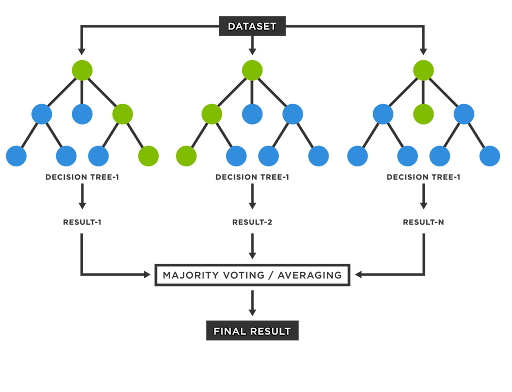
\includegraphics[width=0.5\linewidth]{contents/figures/LR RF diagram.jpg}
    \caption{Random Forest Visualisation \citep{verma_2022}}
    \label{fig:LR RF diagram}
\end{figure}

Training a RF model involves separating the dataset into subsets, and training multiple decision trees on each randomly assigned data subsetm as can be seen in figure \ref{fig:LR RF diagram}. After training, any test data, such as an image of a river and crops, is processed through all the decision trees, each voting on the class, with the average vote determining the final class. 

\begin{itemize}
    \item \textbf{Advantages:}
    \begin{itemize}
        \item Supported by PyCaret and scikit-learn libraries.
        \item The algorithm is logical and well-understood, making it intuitive. 
    \end{itemize}
    \item \textbf{Disadvantages:}
    \begin{itemize}
        \item Required involvement in model development means that this approach is still difficult to manually implement. 
    \end{itemize}
\end{itemize}

\subsubsection{Keras Sequential Model}
More recently, deep learning frameworks such as Keras have enabled the deployment of convolutional neural networks, often built using a simple Sequential model structure, that automatically learn hierarchical feature representations, offering state-of-the-art performance in high-resolution water body extraction challenges. 

Keras models, particularly the sequential model, are known for being one of the simplest ways of training neural networks with TensorFlow \citep{keras-team_2015} and PyTorch \citep{pytorch_2023}. The Keras Sequential model has been used in a TensorFlow tutorial demonstrating capability to classify different images of flowers. The dataset was over over 3,500 images \citep{tensorflow_2018} and after personally testing and adjusting the initially non-functional script to run locally instead of on Google Colab, the model was capable of achieving training data accuracy above 90\% running for 15 epochs. Theoretically, to create another image classification model for a different, bespoke purpose, such as reservoir classification, one would simply have to replace the training and test data used in this tutorial with the training data of their own application. 

\begin{itemize}
    \item \textbf{Advantages:}
    \begin{itemize}
        \item Straightforward implementation.
        \item Step-by-step, pre-made framework outlines all the important steps of model training, simplifying development. 
        \item Highly performant and well suited to image classification. 
    \end{itemize}
    \item \textbf{Disadvantages:}
    \begin{itemize}
        \item Black-box, more difficult to troubleshoot. 
    \end{itemize}
\end{itemize}

\begin{tabular}{@{}l p{0.35\textwidth} p{0.35\textwidth}@{}} 
\toprule
\textbf{Model} & \textbf{Keras Sequential} & \textbf{Random Forest} \\
\midrule
Model Type & Neural Network & Tree-based \\
Structure & Linear stack of layers & Decision Trees \\
Learning & Gradient Descent & Building Trees \\
Feature Learning & Often learns automatically & Uses provided features \\
Interpretability & Lower ("Black Box") & Higher (Feature Importance) \\
Typical Data & Images, Complex Patterns & Tabular, Structured Data \\
Common Library & Keras, TensorFlow & Scikit-learn, PyCaret \\
Core Idea & Hierarchical feature extraction and transformation & Averaging predictions of many diverse trees \\
\bottomrule
\end{tabular}

\subsection{Deep Learning}
Deep learning is a branch of machine learning that trains artificial neural networks with many successive layers to automatically learn large quantities of hierarchical representations of data \citep{nsoft_vision_2023}. Neural networks are named like this because they attempt to simulate the behaviour of the human brain. In a deep neural network, each layer transforms its input (for example, pixel values) into increasingly abstract features (edges, shapes, objects), which is the unique feature of deep neural networks that allow the system to perform complex tasks, such as image recognition from raw inputs. These changes can crucially be made without the programmer strictly coding this behaviour into the model \citep{holdsworth_scapicchio_2024}. 

At its core, a deep learning model consists of multiple “hidden” layers of interconnected "neurons". During training, the network adjusts millions of internal parameters to minimise prediction error on a labelled dataset. Modern architectures, such as convolutional networks for image recognition, build on this principle, enabling breakthroughs higher accuracies for predicting classes \citep{goodfellow_bengio_courville_2016}. These technologies have broader effects in many industries, such as the medical industry to identify tumors \citep{oróstica_mardones_bernal_molina_orchard_verdugo_carvajalhausdorf_marcelain_contreras_armisen_2025}, biological sciences for monitoring growth in organisms, autonomous driving \citep{barla_2021}, and the widespread use of artificial intelligence that operates on similar principles. 

\section{Machine Learning and Classification of Water Bodies}
Machine learning techniques have further enhanced water classification by learning complex spectral and spatial patterns directly from data \citep{ibm_2021b}. The integration of the various different approaches into remote sensing workflows, along with the increased availability of high-resolution satellite imagery has enabled more nuanced discrimination of water features such as "accurate water depth estimation" \citep{liu_wu_wu_zhou_2024} and improved adaptability to varying environmental conditions \citep{rahat_steissberg_etal_2023}.

There has also been research conducted in satellite imagery models being developed specifically for the classification of water reservoirs \citep{ghansah_2022_monitoring}, where the adopted approach was to implement a RF algorithm with no cloud masking required due to low cloud cover. Additionally, given that there is no mention of any spectral indices used for the detection of water, it is implied that the RF model was capable of extracting enough useful information from either a True Colour Image (TCI) or a Red-Green-Blue (RGB) composite to be trained adequately. This means that it appears that spectral indices were not required for effective water detection in Ghana's Upper-East region.

One of the main challenges associated with the study and classification of reservoirs, specifically in east England, is that it can be difficult to properly distinguish between reservoirs and irrigated cropland, waterlogged land, or even trees, as they reflect similar amounts of light in the relevant wavelengths. The approach of omitting the use of spectral water detection indices altogether adopted by \cite{ghansah_2022_monitoring} is one that may be more difficult to implement in this study due to these challenges. 

\subsection{Knowledge Gap}
Despite extensive work on water-index thresholds, machine learning classification, cloud masking, and large-scale water body mapping, no study to date has:
\begin{itemize}
    \item Validated model performance at 10\,m resolution over East England, where vegetation, soil moisture, and irrigation ditches introduce high false-alarm risk due to it being a heavily farmed region.
    \item Integrated end-to-end pipelines (cloud mask $\rightarrow$ water detection $\rightarrow$ classifier) into a single, reproducible workflow and assessed its generalisability across Sentinel-2 revisit cycles under varying seasonal conditions.
\end{itemize}

As a result, it remains unclear which combination of preprocessing and classifier yields robust detection of small agricultural reservoirs at 10m resolution, and how well such a pipeline can scale to routine monitoring for regional water-management agencies. Additionally, there is the informational knowledge gap of there simply not being an accurate register of the number of small reservoirs in the UK. 

Addressing this gap is the central objective of this thesis.